\documentclass{report}

\usepackage[ngerman]{babel}
\usepackage[utf8]{inputenc}
\usepackage[T1]{fontenc}
\usepackage{hyperref}
\usepackage{csquotes}
\usepackage[a4paper]{geometry}
\usepackage{graphicx}



\usepackage[
    backend=biber,
    style=apa,
    sortlocale=de_DE,
    natbib=true,
    url=false,
    doi=false,
    sortcites=true,
    sorting=nyt,
    isbn=false,
    hyperref=true,
    backref=false,
    giveninits=false,
    eprint=false]{biblatex}
\addbibresource{../references/bibliography.bib}


\title{Ethik im Umgang mit Daten}
\author{Eduard Gabrielyan}
\date{\today}


\begin{document}

\maketitle

\abstract{
    Dies ist eine Vorlage für eine Maturarbeit in der Informatik am Gymnasium Muttenz. Sie dient dazu, die Arbeit schnell und einfach zu starten und sollte einen guten Überblick über die Arbeit bieten.
}

\tableofcontents

\chapter{Einleitung}

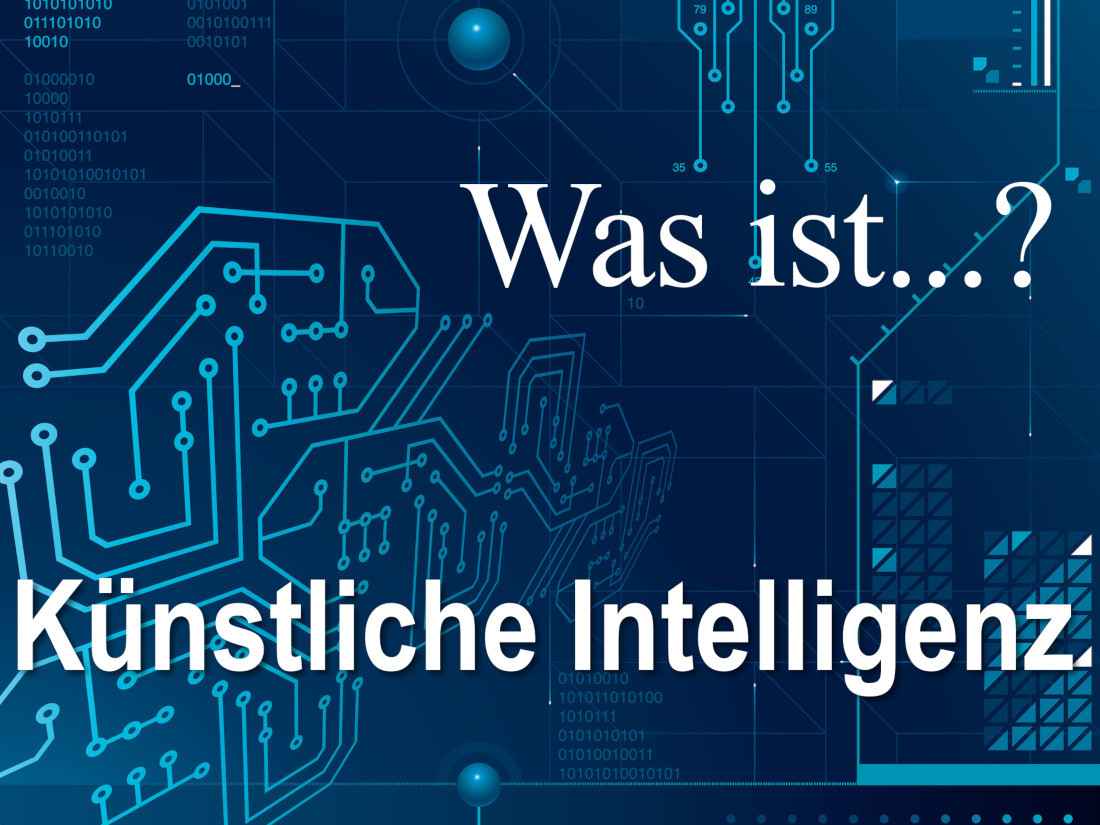
\includegraphics[width=0.4\textwidth]{KI.jpeg}

\section{Was ist KI?}
KI (künstliche Intelligenz) auch Artificial Intelligence AI (English) ist ein sehr wichtiger Teil unserer Gesellschaft geworden.
KI ist Teil der Informatik und beschäftigt sich mit maschinellem Lernen.
In diesem Text geht es darum zu verstehen was KI ist und wie es trainiert wird.
\newline
Künstliche Intelligenz ist wie ein schlauer Computer, der durch Lernen klüger wird. Maschinelles Lernen ist sehr wichtig geworden, da es viele Daten und starke Computer gibt. Dabei lernt der Computer selbst, indem er die Daten anschaut wie Roboter, die lernen Dinge zu greifen und zu bewegen.
\section{Wie wird KI traniert?}
Die Ausbildung einer KI passiert in drei Schritten. Erst bekommt ein Computerprogramm Daten, um vorherzugeben und die Genauigkeit zu überprüfen. Danach wird die Leistung des Programms mit neuen Daten getestet. Es gibt zwei Hauptmethoden beim KI-Training: Beim überwachten Lernen gibt es markierte Eingabe- und Ausgabedaten, beim nicht überwachten Lernen gibt es diese Markierungen eben nicht.
\subsection{Was ist Deep Learning?}
Deep Learning ist ein anstrengender Prozess für den Computer, der viel Rechenleistung braucht und auf einem sehr geschichteten Netzwerk von tiefen neuronalen Pfaden basiert. Jedes Neuron im Netzwerk macht komplexe Muster und Verbindungen durch mathematische Funktionen, die mit Daten gefüttert werden. Deep Learning ist eine Technik des maschinellen Lernens, die es erlaubt Daten zu analysieren und bessere Vorhersagen zu machen.

\subsection{Was ist maschinelles lernen?}
Maschinelles Lernen ist ein Bereich der KI dassAlgorithmen nutzt, um Verbindungen zwischen Variablen zu finden und daraus zu lernen. Mit grossen Datenmengen und viel Rechenleistung können Maschinen Aufgaben selbstständig erlernen und sich verbessern, ähnlich wie Kinder durch Erfahrung lernen. Anders als bei traditionellen Algorithmen folgt maschinelles Lernen keinem vorgegebenen Lösungsweg, sondern die Maschine orientiert sich an einem bestimmten Qualitätskriterium und den Informationen in den Daten. 



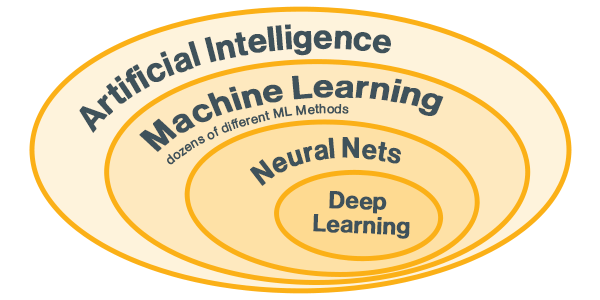
\includegraphics[width=0.5\textwidth]{Training.png}

\section{Gefahren von KI}
Dabei entsteht bei vielen Menschen, die Frage ob KI gefährlich ist. Eigentlich ist Ki selber nicht gefährlich. Die Gefahr kommt vom Missbrauch der Menschen. Wenn wir KI richtig einsetzen und Regeln dafür festlegen, kann sie sehr nützlich sein. Wenn nicht dann gibt es natürlich Gefahren.



\chapter{Unternehmen und KI, Daten, Ethik}
\label{chap:methode}

In diesem Kapitel werde ich auf meine Fragestellung eingehen.
\newline
\textbf{Meine Fragestellung}:
\newline
Wie können Unternehmen ethisch korrekt mit durch KI generierten Daten umgehen?

\vspace{4mm}

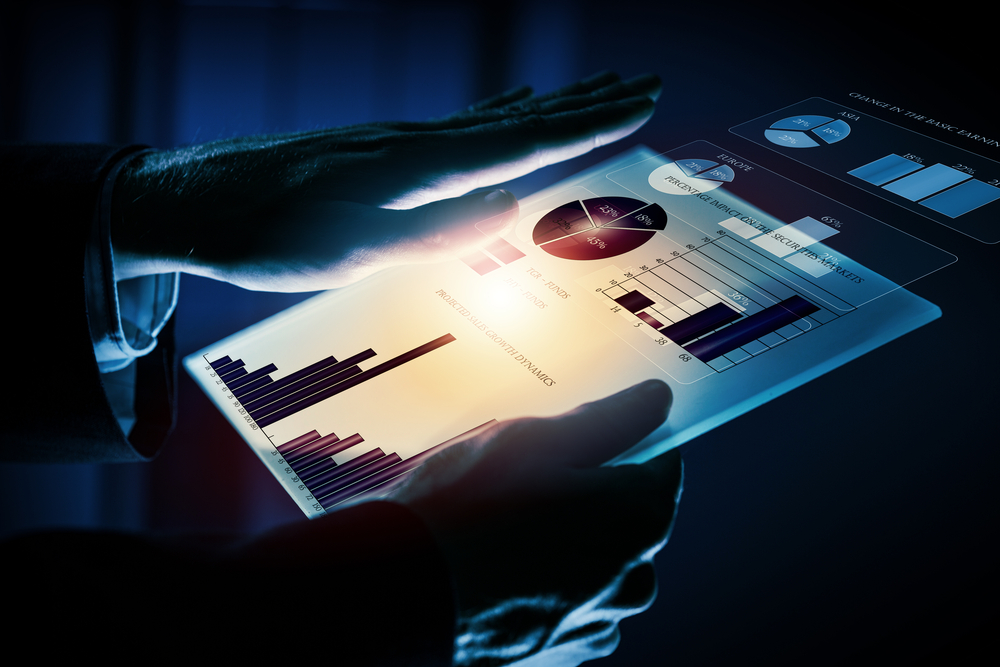
\includegraphics[width=1.0\textwidth]{Verantwortung.jpeg}

\newpage

\section{Verantwortung und Ethik in der KI}
Unternehmen tragen die Verantwortung, eine sichere und transparente KI-Entwicklung zu gewährleisten, Selbstverpflichtungen einzuholen und ethische Prinzipien für den Einsatz von KI-Systemen zu definieren. Sie müssen sicherstellen, dass Kundendaten angemessen verwaltet und geschützt werden und dass Kunden darüber informiert sind, ob sie mit einem Chatbot oder einem echten Menschen sprechen.
\citep{ai-res-cmm360}

\section{Ethischer Umgang mit Daten in Unternehmen}

Unternehmen können sicherstellen, dass sie Daten ethisch verwenden, indem sie Stakeholdern und Mitarbeitern helfen, die ethischen Fragen rund um Daten zu verstehen. Sie sollten klar erklären, wie sie mit Daten umgehen, und moderne Datenschutzlösungen einführen. Storage kann dabei unterstützen, gute Praktiken im Bereich der Datenethik zu verbessern.
\citep{ai-ethik-pure}

\section{Informationspflichten bei KI-generierten Daten}
Unternehmen müssen ihren Kunden klar sagen, wie ihre KI die Daten sammelt, verarbeitet und mit wem diese geteilt werden. Kunden sollten wissen, ob sie mit einem Chatbot oder einem echten Menschen sprechen und welche Rechte sie bei ihren Daten haben. Es ist wichtig, klare  Regeln zu haben, um sicher zu sein, dass die KI ethisch und verantwortungsvoll genutzt wird.
\citep{ai-res-cmm360}

\section{Datenethik}

Datenethik bezieht sich darauf, wie Daten verwaltet, verarbeitet und gespeichert werden, sowie auf moralische Fragen im Zusammenhang mit ihrer Nutzung. Es befasst sich mit der Frage, wie Organisationen Daten auf ethische Weise erfassen, speichern und nutzen können und welche Rechte der Kunden geschützt werden müssen.
\citep{ai-ethik-pure}

\section{Risiken}
Die Risiken von KI sind, dass Unternehmen ein Gleichgewicht zwischen Schnelligkeit und Vertrauen finden müssen, wenn sie KI einführen. Ein Ansatz, der auf Risiken basiert, ist notwendig um Vorteile zu erzielen und Vertrauen aufzubauen. Die ständige Entdeckung von KI-Schwachstellen zeigt, wie anfällig KI-Tools sind. Durch den Einsatz von KI-Tools entstehen neue Sicherheitsrisiken, da KI nicht nur Angreifern hilft, sondern auch neue Arten von Risiken schafft, die beachtet werden müssen.
\citep{ai-risk}

\section{Etwas mit Quellen}

Etwas mit Änderung hier am Ende.

Wenn ich eine Quelle zitieren möchte, kann ich das ganze einfach am Ende des Satzes machen \citep{example}. Oder wie \citet{example} sagt, auch mitten im Text.

\printbibliography

\end{document}
